\section{Розробка алгоритму}

Для побудови прогностичних моделей розроблено та використовується величезна кількість алгоритмів. В загальному вигляді процес використання прогностичних моделей для вхідних даних можна представити у вигляді діаграми на рис. \ref{fig:data_process}.

\begin{figure}[h!]
  \centering
  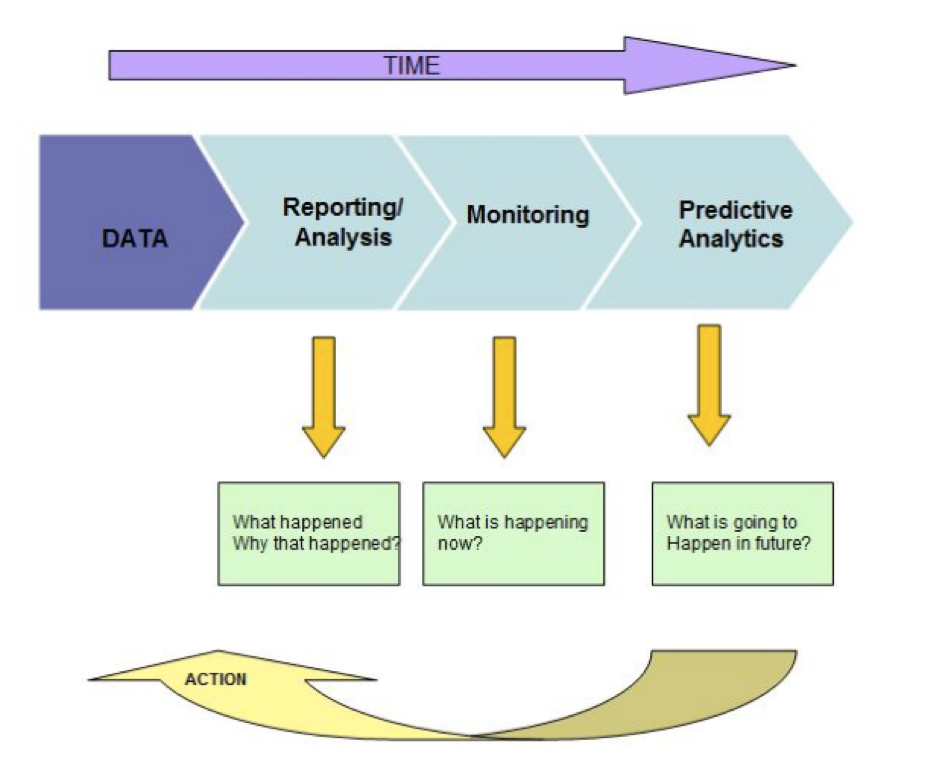
\includegraphics[width=0.7\linewidth]{figures/data_process.png}
  \caption{Процес зміни даних з часом}
  \label{fig:data_process}
\end{figure}

\subsection{Існуючі алгоритми}
Враховуючи те, що результуюча гібридна модель буде використовувати деяку модель в якості базової, доцільно розглянути найбільш поширені алгоритми, що використовуються для класифікації даних. Це дасть змогу зрозуміти головні припципи роботи алгоритмів класифікації, а також за рахунок варіативності даних алгоритмів підкреслити універсальність даного підходу та можливість роботи з будь-якого типу базовими моделями.

\subsubsection{Logistic regression}
В найпростішому випадку опис деякої взаємодії можна звести до двох-трьох категорій змінних за допомогою простих операцій статистики. Проте, в більшості реальних ситуацій потрібно враховувати вплив куди більшої кількості таких змінних, які в загальному випадку можуть бути представлені як багатовимірні таблиці  I × J × K. Саме тому доцільно розглянути узагальнений клас моделей, що носять назву \textit{узагальнених лінійних моделей (\textbf{generalized linear models, GLMs})}. Структурно дані моделі описують шаблони взаємодій та асоціацій. Параметри моделі показують силу таких асоціацій, а основний фокус під час створення таких моделей лягає в оцінку необхідних величин даних параметрів. Узагальнена формула для таких моделей:
\begin{equation}
    \label{eq:logistic_regression}
    y_{i} \sim N(x_{i}^T\beta, \sigma^2)
\end{equation}

Значення вектору $\beta$\ містить коефіцієнти, які і потрібно визначити в ході тренування моделі. В таких моделях значення результуючої змінної підкоряється деякому закону експоненційного розподілу з середнім $\mu_{i}$значенням, який припускається є деякою нелінійною функцією від $x_{i}^T\beta$. Будь-яка модель даного класу містить три основних компоненти:
\begin{itemize}  
	\item Випадковий компонент (\textit{random component}) - відноситься до розподілу ймовірностей результуючої величини $Y$, для лінійної регресії це звичайний нормальний розподіл {Y}. Також носить назву \textit{шуму} або \textit{помилки моделі}.
	\item Систематичний компонент (\textit{systematic component}) - визначає набір додаткових величин $(X_{1}, X_{2}, \ldots X_{k})$ для моделі, а саме їх лінійну комбінацію для створення так званого лінійного провісника (\textit{linear predictor}), наприклад $\beta_{0} + \beta_{1}x_{1} + \beta_{2}x_{2}$ для лінійної регресії.
	\item Зв'язуюча функція (\textit{link function}, $\eta, g(\mu)$) - виражає зв'язок між випадковим та систематичним компонентом. Вона показує, яким чином вихідне значення зв'язане з прогнозованим значенням додаткових величин (наприклад, $\eta = g(E(Y_{i}))=E(Y_{i})$ для лінійної регресії).
\end{itemize}

Загалом серед переваг \textit{GLM}-моделей можна виділити такі:
\begin{itemize}  
	\item не потрібно видозмінювати вихідну величину $Y$, щоб отримати нормальний розподіл;
	\item вибір зв'язуючої функції не залежить від вибору випадкового компоненту, таким чином ми отримуємо більшу гнучкість на етапі моделювання;
	\item якщо зв'язуюча функція адитивна, то нам не потрібно стала дисперсія;
	\item підходи для перевірки моделей є загальними для всіх підвидів класу, тому немає необхідності здійснювати використання окремих інструментів для кожного типу моделі.
\end{itemize}

\subsubsection{Linear Discriminant Analysis}
Linear Discriminant Analysis та Quadratic Discriminant Analysis - два класифікатори, що пропонують лінійну та квадратичну поверхню виборів відповідно. Даного роду алгоритми є досить привабливими, оскільки можуть бути обраховані без додаткових витрат, перевірені на практиці та не мають додаткових метапараметрів для тонкого налаштування.

\begin{figure}[h!]
  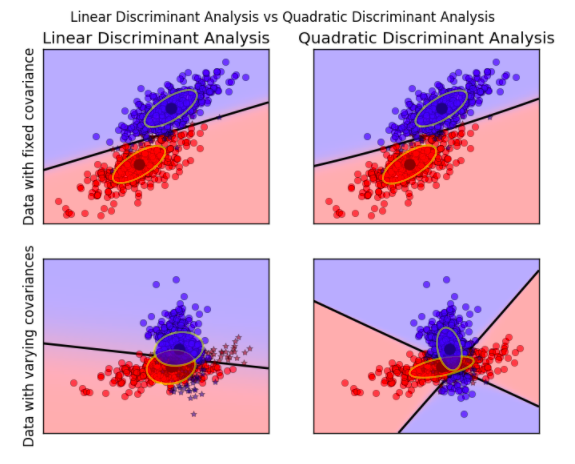
\includegraphics[width=\linewidth]{figures/lda_qda.png}
  \caption{Візуалізація лінійного та квадратичного дискримінантного аналізу}
  \label{fig:lda_qda}
\end{figure}

На рис. \ref{fig:lda_qda} зображено встановлені алгоритмами межі для двох класів. Нижній рядок показує, що лінійний аналіз може здійснити лише лінійний поділ, в той час як квадратичний є більш гнучким. Даний алгоритм часто використовується для зменшення розмірностей простору деякої величини. Він проектує вхідні дані на лінійний підпростір, що максимізує межу поділу між класами. Розмірність вихідних даних завжди менше, ніж кількість класів, тому такий прийом має сенс лише під час виконання мультикласифікації. Обидві моделі унаслідувані від простих ймовірносних моделей на основі умовного розподілу даних $P(X|y  k)$ для кожного класу $k$. Прогнозована величина може бути отримана, використовуючи формулу Байєса:
\begin{equation}
    \label{eq:logistic_regression}
    P(y = k|X) = \frac{P(X|y = k)P(y=k)}{P(X)} = \frac{P(X|y = k)P(y = k)}{\sum_{l}P(X|y=l) \cdot P(y=l)}
\end{equation}

Потім ми обираємо клас $k$, який максимізує умовну ймовірність. Щоб використовувати дану дану модель в якості класифікатора необхідно визначити з вхідних тренувальних даних такі величини: $P(y=k)$ - відношення екземплярів для класу $k$, середні значення для класу $\mu_{i}$ та коваріативну матрицю. У випадку, якщо кількість вхідних даних для тренування досить мала в порівнянні з кількість незалежних змінних датасету (\textit{features}), можна скористатися параметром \textit{усадки} (\textit{shrinkage}). Це значення в межах від 0 до 1, де 1 означає, що діагональна матриця дисперсії буде використана для обрахунку коваріативної матриці. Використання усадки на вхідних даних дає змогу збільшити точність класифікації для варіанту, згаданого вище (рис. \ref{fig:shrinkage}).

\begin{figure}[h!]
  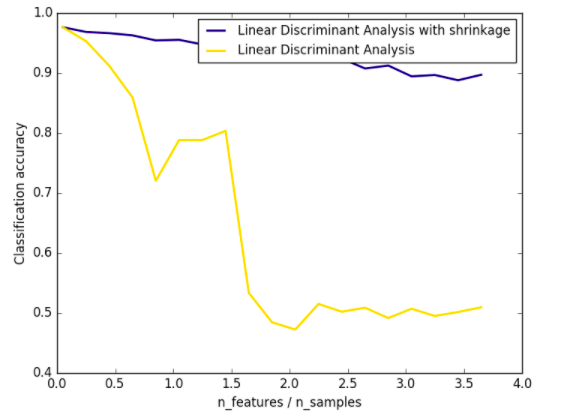
\includegraphics[width=\linewidth]{figures/shrinkage.png}
  \caption{Показники точності з використання усадки та без неї}
  \label{fig:shrinkage}
\end{figure}

\subsubsection{Gaussian Naive Bayes}
Наївні Байєсівські методи - це набір методів, що використовуються для навчання з учителем та ґрунтуются на застосуванні теореми Байєса з "наївним" припущенням, що кожна пара колонок вхідного датасету (\textit{features}) є незалежною між собою. Маючи змінну класу та залежний вектор характеристичних величин, теорема Байєса відображає таку залежність 
\begin{equation}
    \label{eq:naive_bayes_0}
    P(y|x_{1}, \ldots, x_{n}) = \frac{P(y)P(x_{1}, \ldots, x_{n}|y)}{P(x_{1}, \ldots, x_{n})}
\end{equation}

Припускаючи незалежність величин
\begin{equation}
    \label{eq:naive_bayes_1}
    P(x_{i}|y, x_{1}, \ldots, x_{i-1}, x_{i+1}, \ldots, x_{n}) = P(x_{i}|y)
\end{equation}

для всіх $i$-тих елементів, дане відношення можна спростити до вигляду
\begin{equation}
    \label{eq:naive_bayes_2}
    P(y|x_{1}, \ldots, x_{n}) = \frac{P(y)\prod_{i=1}^n P(x_{i}|y)}{P(x_{i}, \ldots, x_{n})}
\end{equation}

З даної формули тепер можна вивести таке правило для класифікації:
\begin{equation}
    \label{eq:naive_bayes_3}
    \hat{y} = \underset{y}{argmax}P(y)\prod_{i=1}^n P(x_{i}|y)
\end{equation}

Одним з часто використовуваних підвидів Байєсівського класифікатора є класифікатор з використанням розподілу Гауса:
\begin{equation}
    \label{eq:naive_bayes_4}
    P(x_{i}|y) = \frac{1}{\sqrt{2\pi\sigma_{y}^2}}exp(-\frac{(x_{i}-\mu_{y})^2}{2\sigma_{y}^2})
\end{equation}

Різні підвиди наївного Байєсівського класифікатора відрізняються в основному припущеннями, які вони здійснюють стосовно розподілу $P(x_{i}|y)$. Незважаючи на використання таких занадто спрощених припущень, наївні Байєсівські класифікатори дуже добре працюють в багатьох реальних прикладних ситуаціях. Велика кількість класифікаторів документів, а також спам-фільтрів побудована саме на такого роду класифікаторах. Вони вимагають невеликої кількості вхідних даних для тренування та швидко встановлюють необхідні параметри. Ще однією з переваг є те, що такі класифікатори показують високу швидкодію в порівнянні з більш складними методами.


\subsubsection{Support Vector Machines}
Support Vector Machines - це також множина методів, що використовуються для класифікації, а також для визначення аномалій вхідних даних. Основними перевагами для використання цих методів є такі:
\begin{itemize}  
	\item ефективність в багатовимірних просторах;
	\item непогані показники навіть за умов, коли кількість розмірностей більша за кількість екземплярів;
	\item використання підмножини точок тренувального набору в якості функції рішення, що робить алгоритм ефективним з точки зору використання пам'яті;
	\item різносторонність: в якості функції рішення можна вибрати велику кількість уже існючих або використати будь-яку свою.
\end{itemize}

Щодо недоліків цих методів включають:
\begin{itemize}  
	\item низька швидкодія за умови, коли кількість характеристичних ознак набагато більша за кількість зразків;
	\item сам метод не надає жодних функцій для оцінки ймовірностей та вимагає додаткового кроку крос-валідації
\end{itemize}

В якості функції рішення (\textit{kernel function}) можна обрати будь-яку з наведених:
\begin{itemize}  
	\item linear: $\langle x, x'\rangle$;
	\item polynomial: ($\gamma\langle x, x'\rangle + r)^d$;
	\item rbf: $exp(-\gamma|x-x'|^2)$;
	\item sigmoid: $tanh(\gamma\langle x, x'\rangle + r)$.
\end{itemize}

З математичної точки зору даний метод будує гіперплощину чи множину гіперплощин в багаторозмірному просторі, які потім використовуються для класифікації. 

\begin{figure}[h!]
  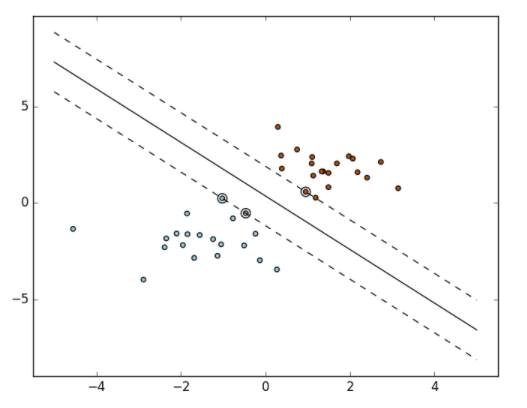
\includegraphics[width=\linewidth]{figures/svm.png}
  \caption{Знаходження межі та поділ на класи}
  \label{fig:svm}
\end{figure}

Поділ на класи виконується за рахунок знаходщення такої гіперплощини (рис. \ref{fig:svm}), що дає найбільшу відстань між найближчими точками з тренувального набору даних будь-якого класу, оскільки чим більша межа, тим мена помилка узагальнення для класифікатора. Для класифікації використовується така функція вибору:
\begin{equation}
    \label{eq:svc}
    sgn(\sum_{i=1}^n y_{i}\alpha_{i}K(x_{i}, x)+\rho)
\end{equation}

\subsubsection{Decision Tree Classifier}
Дерева вибору (\textit{decision trees}) - набір непараметризованих методів для машинного навчання з учителем, що використовуються для класифікації. Метою є створення такої моделі, що буде передбачати значення досліджуваної величини на основі простого набору правил, виведених з даних характерестичних величин. Приклад на рис. показує як за допомогою дерев вибору здійснити апроксимацію синусоїди за допомогою набору правил \textit{"якщо-тоді-інакше"}. Чим більше рівнів у дерева, тим більша кількість правил і тим точнішою є модель.

\begin{figure}[h!]
  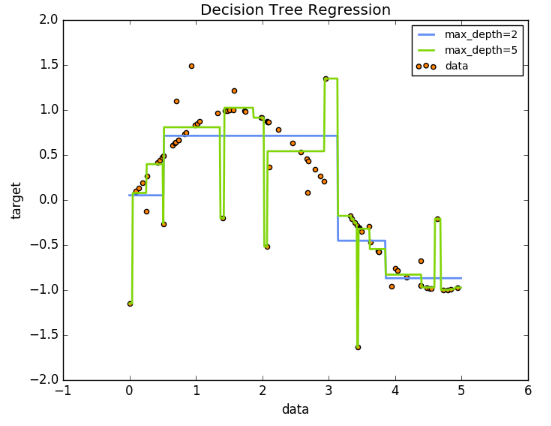
\includegraphics[width=\linewidth]{figures/decision_trees.png}
  \caption{Апроксимація синусоїди деревом вибору}
  \label{fig:decision_trees}
\end{figure}

Серед переваг використання дерев вибору виділимо такі:
\begin{itemize}  
	\item простота розуміння та інтерпретації;
	\item можливість простої візуалізації;
	\item майже не вимагає попередньої підготовки даних; нормалізація чи видалення порожніх значень можуть бути пропущені;
	\item логарифмічна складність алгоритму;
	\item можливість роботи як з числовими, так і з нечисловими даними;
	\item використання у алгоритмах, що потребують множинних відповідей;
	\item використання моделі \textit{white box} (відкритої коробки): обґрунтування вибору моделі може бути виведене звичайною булевою алгреброю, в той час як рішення інших моделей (наприклад, нейронних мереж) може бути складним для пояснення і розуміння людиною;
	\item можливість валідації моделі, використовуючи лише статистичні перевірки;
	\item показує гарні результати, навіть якщо припущення у деяких умовах є хибними.
\end{itemize}

Хоча дерева вибору і мають велику кількість переваг, на противагу їм є і достатня кількість недоліків:
\begin{itemize}  
	\item навчаючись, модель може створити занадто громіздке дерево, яке насправді не зможе гарно узагальнити вхідні дані. Також можливий ефект надмірної точності (\textit{overfitting}), коли модель занадто добре працює на вхідних даних, але показує незадовільні результати для будь-яких інших даних;
	\item дерева можуть бути нестабільними, оскільки навіть невелика зміна чи відхилення у вхідних даних призводить до побудови зовсім іншого дерева. Даний проблема вирішується використанням іншого класу алгоритмів на основі множини дерев.
	\item для того, щоб створити оптимальне дерево вибору потрібно вирішити \textit{NP}-повну задачу, а це означає, що ми не завжди отримаємо найкращий результат, оскільки потрібно використовувати жадібні алгоритми чи евристики;
	\item дерева вибору схильні давати упереджені результати, якщо деякий клас є домінуючим. Результати передбачення будуть зміщені в сторону домінуючого класу. Щоб вирішити таку проблему використовують попередню обробку чи балансування вхідних даних.
\end{itemize}

Критерій класифікації, що застосовується для дерев вибору, виражається так:
\begin{equation}
    \label{eq:decision_trees}
    p_{mk} = 1/N_{m}\sum_{x_{i} \in R_{m}}I(y_{i}=k)
\end{equation}

Це буде виражати пропорцію входжень деякого класу $k$ у вузлі $m$. Для визначення похибки користуются формулою:
\begin{equation}
    \label{eq:gini_norm}
    H(X_{m})=\sum_{k}p_{mk}(1-p_{mk})
\end{equation}

\subsubsection{K Nearest Neighbours}
Алгоритми групи "найближчих сусідів" можуть бути використані для машинного навчання як з учителем, так і без нього. Методи даного класу дуже часто застосовуються в кластеризація та є базою для багатьох інших методів. Основний принцип даних алгоритмів дуже простий - знайти визначену кількість входжень серед заданого вхідного набору даних (сусідів), що мають найменшу відстань до вибраної нової точки і на основі цього віднести її до того ж самого класу. Кількість таких входжень регулюється деякою константою $k$, звідси і назва алгоритму. Відстань може бути як і звичайною Евклідовою відстанню (що використовується найчастіше), так і будь-якою іншою метрикою для довільного простору. Незважаючи на простоту алгоритму, він використовується під час вирішення досить складних задач, таких як розпізнавання рукописного тексту чи знімків супутника. Метод є непараметризованим, а тому використовується в ситуаціях, коли межа поділу між класами досить нечітка і непостійна.

Для класифікації на основі цього алгоритму достатньо більшості голосів для кожної точки, тобто знаходження найбільшої кількості екземплярів деякого класу серед вибраної кількості сусідів. Значення буде віднесено до того класу, який містить найбільшу кількість представників серед вибраних найближчих сусідів. Якщо вхідні дані 
розподілені нерівномірно, доцільно обрати не наперед визначену кількість сусідніх точок, а деякий радіус $r$, та розглянути всі точки, що потрапляють в отриману множину.

Також інколи доцільно застосовувати "зважений" метод. Це модифікація яка надає деяке значення ваги кожному з сусідів. У найпростішому випадку вагою може бути коефіцієнт від відстані: чим ближче точка-сусід знаходиться до нашої цільової точки, тим більше значення ваги вона матиме. Для ваги можна визначити будь-яку користувацьку функцію, що робить алгоритм досить гнучким і дозволяє більш точно визначити межі класів.

\begin{figure}[h!]
  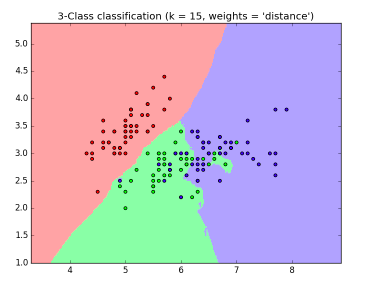
\includegraphics[width=\linewidth]{figures/knn.png}
  \caption{Класифікація методом найближчих сусідів для трьох класів}
  \label{fig:knn}
\end{figure}

Щоб зробити знаходження найближчих сусідів швидким процесом продиться велика кількість досліджень, оскільки найпростіший спосіб зводиться до повного перебору та обчислення відстаней до всіх точок. Для $N$ точок в $D$ вимірному просторі це вимагає порядку $O[DN^2]$ операцій, що прийнятно лише для невеликої кількості точок. Наразі існують підходи на основі дерев, що дозволяють зробити пошук дещо швидшим: \textit{K-D Tree} та \textit{Ball Tree}.

\subsection{Оптимізація алгоритмів для використання у предметній галузі}
Оскільки велика кількість алгоритмів вимагають специфічного середовища чи платформи, а для побудови інших необхідні значні обчислювальні потужності, постає проблема платформозалежності та неможливості використання кращих підходів за умови існування додаткових обмежень. Щоб уникнути даних проблем, достатньо розробити рішення, що буде відповідати поставленим нижче вимогам:
\begin{itemize}  
	\item доступ користувача до коду моделі на будь-якій платформонезалежній мові, що дозволить запускати її в довільному середовищі та не спиратися на використання сторонніх бібліотек;
	\item будова моделі та деталі її внутрішньої реалізації повинні бути відкритими, тобто користувач повинен мати змогу переглянути вихідний код і в разі необхідності самостійно відтворити довільний крок та отримати аналогічний результат передбачення для однакового набору вхідних даних;
	\item модель повинна мати точність максимально наближену до точності моделей, що показують найкращі результати для вибраних вхідних даних. Модель повинна мати аналогічні показники щонайменше для 95\% всіх вхідних наборів даних;
	\item виконання коду програми повинно бути швидким (близько 1 мс на рядок вхідних даних).
\end{itemize}

Єдиного рішення, що дозволило б відмовитися від наявних алгоритмів на користь одного, визначеного вимогами вище, поки що немає, але існує підхід, що дозволяє покрити перелік всіх умов. Даний підхід носить назву апроксимаційної моделі. Основна ідея полягає в припущенні, що деяка відносно проста модель, побудована на основі передбачень більш складної моделі може показати схожі результати в межах допустимого відхилення. Саме такою моделлю є RuleFit-модель, або модель на основі класу визначених правил. Принцип роботи полягає в серії тренувань дерев вибору на вхідних даних з наступною конвертацією гілок дерев в класи правил. Наприклад, одне правило може виражатися такою формулою: $20 < age <= 30 and income > 10000$. Новий набір даних створюється на основі оригінальних вхідних даних, генеруючи набір індикаторів $0/1$ таким чином, що кожен рядок позначає негативне чи позитивне значення в залежності від результату застосування правила до цього рядка. Дані індикатори потім використовуються в якості значень передбачення для узагальненої лінійної моделі.
\begin{equation}
    \label{eq:linear_model}
    y(w, x) = w_{0} + w_{1}x_{1} + \ldots + w_{p}x_{p}
\end{equation}

Формула \ref{eq:linear_model} описує звичайну модель, що є лінійною комбінацією вхідних значень та вектора коефіцієнтів $w$, а  $y$ – це значення, для якого здійснюється передбачення.

RuleFit є простою моделлю в тому плані, що це лише список правил з відповідними коефіцієнтами для кожного з них. Однак існують і недоліки, пов'язані з тим, що класи правил можуть містити подібні правила, що ускладнює інтуїтивне розуміння впливу коефіцієнтів, тобто вносить складність для розуміння людиною.

Існує дві основних частини в реалізації алгоритму: безпосереднє тренування і передбачення та rulefit задача. Дана задача містить багато параметрів, найголовнішим з яких є альфа-параметр, що визначає розмір регуляризації, що застосовується до лінійної моделі RuleFit.

Кінцевим етапом стоврення такої моделі повинна бути валідація згенерованого коду. Оскільки немає жорсткої прив’язки до використовуваної мови, потрібно переконатися, що код компілюється та виконується коректно. Далі потрібно запустити код та зберегти файл з прогнозованими значеннями для подальшого порівняння зі значеннями, що отримуються від оригінальної моделі. Якщо похибка лежить в межах допустимого відхилення валідація вважається успішно пройденою.

